\documentclass[letterpaper]{l3doc}

\hypersetup{urlcolor = teal, filecolor = violet}
\usepackage[mono = false]{libertine}
\usepackage{pdfpages,hologo,framed}
\hologoFontSetup{general = \sffamily}
\FrameSep = 0pt
\usepackage[fontset = none]{ctex}
\setCJKmainfont[BoldFont = *-Medium]{LXGW WenKai}
\setCJKsansfont[BoldFont = *-Medium]{LXGW WenKai}
\setCJKmonofont[BoldFont = *-Medium]{LXGW WenKai Mono}
\usepackage[os = mac]{menukeys}
\AddToHook{env/function/before}{\vspace{-.3\baselineskip}}
\AddToHook{env/syntax/after}{\vspace{-.2\baselineskip}}

\title
{
  \bfseries\cls{litetable} 文档类:多彩的课程表
  \thanks{\url{https://github.com/xiamyphys/litetable}}
}
\author
{
  夏明宇 \texttt{<\href{mailto:xiamyphys@gmail.com}{xiamyphys@gmail.com}>}
  \thanks{\href{https://github.com/ljguo1020}{郭李军}开发了读取 \meta{left} -> \meta{right} 型数据结构模块和低版本 \hologo{TeX} Live 兼容模块.}
}
\date{Version 3.1D, \today}

\begin{document}

\maketitle

\section{介绍}

\cls{litetable} 文档类提供了一个多彩的课程表设计,基于 \cls{article} 文档类,由 \pkg{expl3} 和 \pkg{tikz} 构建. 兼容发行版 \hologo{TeX} Live 2019 及更高版本,在 \hologo{pdfLaTeX} 和 \hologo{XeLaTeX} 编译器下均可正常运行. 本文档为 \cls{litetable} 文档类的中文用户手册,手册同时有 \href{./litetable-en.pdf}{英文} 和 \href{./litetable-hk.pdf}{粤语} 版本\footnote{\href{https://qm.qq.com/q/RyssAhG4qy}{QQ Group: 760570712}}.

\section{载入 \cls{litetable} 并生成课程表框架}

同加载其他文档类一样,只需写下

\begin{framed}
  \begin{verbatim}
    \documentclass {litetable}
  \end{verbatim}
\end{framed}

如需输入中文,可自行载入 \pkg{ctex} 宏包并设置字体.

\begin{function}{\timelist,\weeklist}
  \begin{syntax}
    \cs{timelist} \oarg{rows} \marg{list}            \cs{timelist} \marg{list} \oarg{rows}
    \cs{weeklist} \oarg{default weeks} \marg{list}   \cs{weeklist} \marg{list} \oarg{default weeks}
  \end{syntax}

  命令 \cs{timelist} 的可选参数可强制设定课程表的行数,命令 \cs{weeklist} 的可选参数可设定默认的星期数目并会在每个课程盒子的右下角显示. 两个命令的强制参数均接收数组,可分别在课程表的左侧添加时间列表、在课程表的顶部添加对应宽度比例的工作日. 输入数组的用例见Appendix \ref{mwe}.

  若命令 \cs{timelist} 中时间数组数大于强制设定的行数,则多余的时间数组将被忽略,并返回一个警告. 如果只需在课程表左侧添加一列序号,使强制参数为空即可.
\end{function}

\begin{function}{\more}
  \begin{syntax}
    \cs{more} \marg{comment}
  \end{syntax}

  此命令可在页面的右下角添加备注.
\end{function}

\begin{function}{\maketable}
  \begin{syntax}
    \cs{maketable} \oarg{keyvals} \marg{title} \oarg{keyvals}
  \end{syntax}

  此命令可生成一个空白的课程表框架,需在命令 \cs{timelist},\cs{weeklist} 和 \cs{more} 后,并在带有 \cmd{[remember picture, overaly]} 选项的 \env{tikz} 环境中执行. 可选参数接收键 \keys{\cmdmac~color} \keys{\cmdmac~sem},可分别在设置课程表框架的背景色和在页面的右上角添加学期,键 \keys{\cmdmac~color} 的默认值为 \cmd{gray}. 强制参数可设定标题.
\end{function}

\section{添加课程盒子}

\begin{function}{\course}
  \begin{syntax}
    \cs{course} \oarg{keyvals} \marg{start number} \oarg{keyvals} \marg{end number} \oarg{keyvals}
  \end{syntax}

  \cs{course} 命令可在当前工作日添加课程盒子,需在命令 \cs{maketable} 后,并在带有 \cmd{[remember picture, overaly]} 选项的 \env{tikz} 环境中执行.
  
  此命令的可选参数接收下列键:\keys{\cmdmac~color} \keys{\cmdmac~subject} \keys{\cmdmac~location} \keys{\cmdmac~teacher} \keys{\cmdmac~weeks}. 键 \keys{\cmdmac~color} 默认值为 \cmd{teal},键 \keys{\cmdmac~weeks} 默认值由命令 \cs{weeklist} 的可选参数设定. 第一个和第二个强制参数分别为课程的开始和结束序号. 命令的用例见Appendix \ref{mwe}.
  
  \begin{itemize}
    \item 若课程盒子的高度只有一格,即$\meta{start number} = \meta{end number}$,则键 \keys{\cmdmac~location} 和 \keys{\cmdmac~teacher} 的值将输出在同一行并以逗号 (,) 间隔,键 \keys{\cmdmac~weeks} 的值将会隐藏.
    \item 若键 \keys{\cmdmac~location} 和 \keys{\cmdmac~teacher} 均未赋值,则键 \keys{\cmdmac~subject} 的值将输出在课程盒子中心.
    \item 超出课程表工作日范围的课程盒子将不会显示,并返回一条警告.
  \end{itemize}
\end{function}

\begin{function}{\newday}
  \begin{syntax}
    \cs{newday} \oarg{integral value}
  \end{syntax}

  此命令可使其后面添加的课程盒子后移 \meta{intergal value} 个工作日. 可选参数的默认值为 \cmd{1},即后移 \cmd{1} 个工作日.
\end{function}

\clearpage
\appendix

\section{最小工作示例}\label{mwe}

此MWE生成的课程表有13行但是只有前12行标注时间,课程表顶部共有5个工作日,工作日之间的宽度比例为$4:5:4:6:5$,键 \keys{\cmdmac~weeks} 的默认值被赋为 \cmd{Weeks 1 - 16}. 添加了注释和两个课程盒子.

\begin{framed}
  \begin{verbatim}
    \documentclass{litetable}

    \begin{document}

    \timelist [ 13 ]
      {
        08:05 -> 08:50, 08:55 -> 09:40, 10:00 -> 10:45, 10:50 -> 11:35,
        11:40 -> 12:25, 13:30 -> 14:15, 14:20 -> 15:05, 15:15 -> 16:00,
        16:05 -> 16:50, 18:30 -> 19:15, 19:20 -> 20:05, 20:10 -> 20:55
      }
    \weeklist [ Weeks 1 - 16 ]
      {
        Mon -> 4, Tue -> 5, Wed -> 4, Thu -> 6, Fri -> 5
      }
    \more { Author: Mingyu Xia \& Lijun Guo }

    \begin{tikzpicture} [ remember picture, overlay ]
      \maketable
      \course [ subject = Keep on {\TeX}ing ] {10} {11}
      \newday
      \course [ color = DarkSlateGray, subject = litetable,
                location = Hong Kong, teacher = M.Y. Xia
              ] {8} {8}
    \end{tikzpicture}

    \end{document}
  \end{verbatim}
\end{framed}

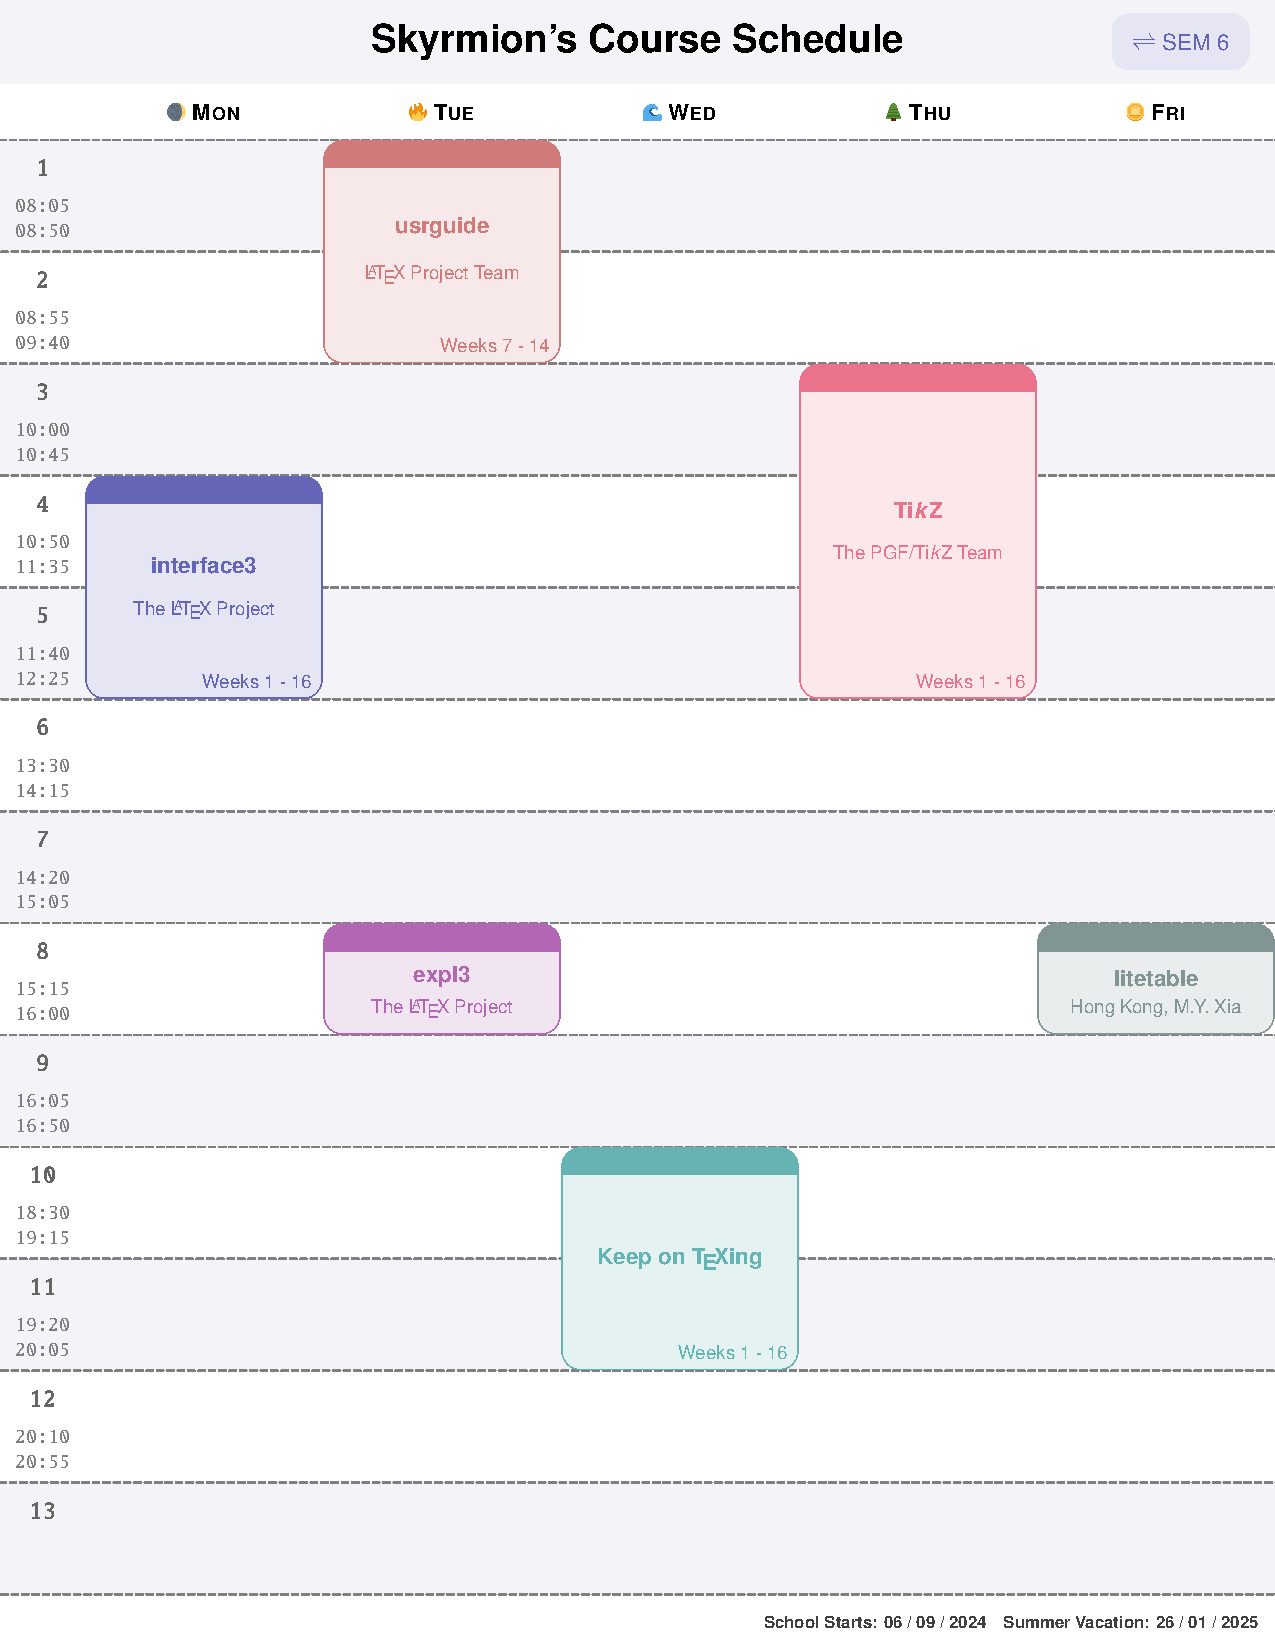
\includepdf[pages = 1]{litetable-demo.pdf}

\end{document}

% End of file litetable-cn.tex
